\documentclass[11pt]{article}
\usepackage[T1]{fontenc}
\usepackage[utf8]{inputenc}
\usepackage{lmodern}
\usepackage[margin=1in]{geometry}
\usepackage{amsmath,amssymb}
\usepackage{booktabs}
\usepackage{xcolor}
\usepackage{graphicx}
\usepackage{float}
\usepackage[font=small,labelfont=bf]{caption}
\usepackage{subcaption}
\usepackage[authoryear,round]{natbib}
\usepackage[colorlinks=true,linkcolor=blue!50!black,citecolor=blue!50!black,urlcolor=blue!50!black]{hyperref}
\usepackage{enumitem}
\setlist{nosep,leftmargin=*}

% Auto-generated by scripts/run_all.py -- do not edit.
\newcommand{\ApxCapmAlpha}{7.00}
\newcommand{\ApxCapmT}{2.52}
\newcommand{\ApxFfAlpha}{7.04}
\newcommand{\ApxFfT}{5.22}
\newcommand{\BaseRankIS}{2}
\newcommand{\BearAlpha}{5.92}
\newcommand{\BearMean}{4.75}
\newcommand{\BearMktBeta}{-0.01}
\newcommand{\BearMonths}{175}
\newcommand{\BearUmdBeta}{0.82}
\newcommand{\BgAlpha}{0.19}
\newcommand{\BgT}{2.86}
\newcommand{\BreakEvenAlpha}{26}
\newcommand{\BreakEvenMean}{82}
\newcommand{\BullAlpha}{1.68}
\newcommand{\BullMean}{10.01}
\newcommand{\BullMktBeta}{0.05}
\newcommand{\BullUmdBeta}{0.85}
\newcommand{\CorrCapmAlphaRep}{0.98}
\newcommand{\CorrFfAlphaRep}{0.92}
\newcommand{\CorrMktHml}{-0.36}
\newcommand{\CorrMktSmb}{0.37}
\newcommand{\CorrSmbHml}{-0.09}
\newcommand{\CostBps}{25}
\newcommand{\CostTwoSig}{5}
\newcommand{\DevCapmAlpha}{5.34}
\newcommand{\DevCapmT}{3.07}
\newcommand{\DevFfAlpha}{4.50}
\newcommand{\DevFfT}{7.25}
\newcommand{\DsrBase}{0.997}
\newcommand{\DsrBest}{0.999}
\newcommand{\EndSample}{August 2026}
\newcommand{\EurCapmAlpha}{3.54}
\newcommand{\EurCapmT}{2.04}
\newcommand{\EurFfAlpha}{2.34}
\newcommand{\EurFfT}{3.82}
\newcommand{\ExpMean}{8.81}
\newcommand{\GridBest}{$L=12$, skip $=0$, $n=10$}
\newcommand{\GridBestAlphaOOS}{2.93}
\newcommand{\GridBestSharpeIS}{0.89}
\newcommand{\GridBestSharpeOOS}{0.40}
\newcommand{\GridBestTOOS}{1.96}
\newcommand{\GridMedianSharpeOOS}{0.32}
\newcommand{\GridN}{16}
\newcommand{\GridRho}{0.72}
\newcommand{\GrsCapmIS}{1.98}
\newcommand{\GrsCapmISp}{0.004}
\newcommand{\GrsFfFull}{3.64}
\newcommand{\GrsFfFullp}{0.0000}
\newcommand{\GrsFfIS}{1.43}
\newcommand{\GrsFfISp}{0.086}
\newcommand{\GrsFfOOS}{3.71}
\newcommand{\GrsFfOOSp}{0.000}
\newcommand{\GrsFfTdIS}{1.54}
\newcommand{\GrsFfiveFull}{3.23}
\newcommand{\GrsFfiveFullp}{0.0000}
\newcommand{\GrsTdIS}{2.05}
\newcommand{\HedCapmAlpha}{2.70}
\newcommand{\HedCapmT}{2.12}
\newcommand{\HedFfAlpha}{2.60}
\newcommand{\HedFfT}{2.02}
\newcommand{\HedFfUmdAlpha}{2.56}
\newcommand{\HedFfUmdT}{1.97}
\newcommand{\HedFfiveAlpha}{2.74}
\newcommand{\HedFfiveT}{2.16}
\newcommand{\HedFfiveUmdAlpha}{2.74}
\newcommand{\HedFfiveUmdT}{2.08}
\newcommand{\HedMean}{2.64}
\newcommand{\HedSharpe}{0.28}
\newcommand{\HedVol}{9.40}
\newcommand{\HiVolMean}{6.16}
\newcommand{\HmlCorr}{1.0000}
\newcommand{\HmlMeanIS}{0.38}
\newcommand{\HmlRmse}{0.29}
\newcommand{\HmlTIS}{2.75}
\newcommand{\ImomCapmAlpha}{9.40}
\newcommand{\ImomCapmAlphaIS}{11.79}
\newcommand{\ImomCapmAlphaOOS}{7.75}
\newcommand{\ImomCapmR}{0.01}
\newcommand{\ImomCapmT}{4.90}
\newcommand{\ImomCapmTIS}{4.34}
\newcommand{\ImomCapmTOOS}{2.94}
\newcommand{\ImomFfAlpha}{10.78}
\newcommand{\ImomFfAlphaIS}{13.27}
\newcommand{\ImomFfAlphaOOS}{8.88}
\newcommand{\ImomFfR}{0.05}
\newcommand{\ImomFfT}{5.75}
\newcommand{\ImomFfTIS}{5.11}
\newcommand{\ImomFfTOOS}{3.46}
\newcommand{\ImomFfUmdAlpha}{2.31}
\newcommand{\ImomFfUmdAlphaIS}{1.43}
\newcommand{\ImomFfUmdAlphaOOS}{1.87}
\newcommand{\ImomFfUmdR}{0.67}
\newcommand{\ImomFfUmdT}{2.09}
\newcommand{\ImomFfUmdTIS}{0.84}
\newcommand{\ImomFfUmdTOOS}{1.31}
\newcommand{\ImomFfiveAlpha}{10.42}
\newcommand{\ImomFfiveR}{0.05}
\newcommand{\ImomFfiveT}{4.92}
\newcommand{\ImomFfiveUmdAlpha}{2.76}
\newcommand{\ImomFfiveUmdAlphaIS}{1.82}
\newcommand{\ImomFfiveUmdAlphaOOS}{2.26}
\newcommand{\ImomFfiveUmdR}{0.67}
\newcommand{\ImomFfiveUmdT}{2.46}
\newcommand{\ImomFfiveUmdTIS}{0.98}
\newcommand{\ImomFfiveUmdTOOS}{1.60}
\newcommand{\ImomHmlBetaFf}{-0.30}
\newcommand{\ImomMaxDD}{-53}
\newcommand{\ImomMean}{8.63}
\newcommand{\ImomMeanIS}{11.67}
\newcommand{\ImomMeanOOS}{6.13}
\newcommand{\ImomMktBetaCapm}{-0.11}
\newcommand{\ImomNetMean}{6.01}
\newcommand{\ImomNetSharpe}{0.39}
\newcommand{\ImomSharpe}{0.56}
\newcommand{\ImomSharpeIS}{0.81}
\newcommand{\ImomSharpeOOS}{0.38}
\newcommand{\ImomSkew}{-0.76}
\newcommand{\ImomT}{4.46}
\newcommand{\ImomUmdBeta}{0.87}
\newcommand{\ImomVol}{15.38}
\newcommand{\IntlNCapmSig}{4}
\newcommand{\IntlNFfSig}{5}
\newcommand{\IntlStart}{July 1990}
\newcommand{\JpnCapmAlpha}{4.45}
\newcommand{\JpnCapmT}{1.99}
\newcommand{\JpnFfAlpha}{2.60}
\newcommand{\JpnFfT}{3.84}
\newcommand{\LoVolMean}{11.21}
\newcommand{\MadFfAlphaRep}{0.04}
\newcommand{\MeanAbsCapmAlpha}{0.26}
\newcommand{\MeanAbsFfAlpha}{0.09}
\newcommand{\MktMean}{7.22}
\newcommand{\MktMeanIS}{0.41}
\newcommand{\MktSharpe}{0.47}
\newcommand{\MktTIS}{1.65}
\newcommand{\NCapmFfHolm}{15}
\newcommand{\NCapmFfTests}{28}
\newcommand{\NCapmRNinety}{2}
\newcommand{\NFfRNinety}{22}
\newcommand{\NFull}{758}
\newcommand{\NIS}{342}
\newcommand{\NTests}{90}
\newcommand{\NUmdHolm}{0}
\newcommand{\NUmdTests}{62}
\newcommand{\NUmdThree}{0}
\newcommand{\NUmdTwo}{9}
\newcommand{\NaCapmAlpha}{3.68}
\newcommand{\NaCapmT}{1.49}
\newcommand{\NaFfAlpha}{3.92}
\newcommand{\NaFfT}{5.18}
\newcommand{\NetCapmAlpha}{6.78}
\newcommand{\NetCapmT}{3.51}
\newcommand{\NetFfAlpha}{8.17}
\newcommand{\NetFfT}{4.32}
\newcommand{\NetFfUmdAlpha}{-0.31}
\newcommand{\NetFfUmdT}{-0.28}
\newcommand{\NetFfiveAlpha}{7.81}
\newcommand{\NetFfiveT}{3.66}
\newcommand{\NetFfiveUmdAlpha}{0.14}
\newcommand{\NetFfiveUmdT}{0.12}
\newcommand{\PostTwoKAlphaFfUmd}{1.92}
\newcommand{\PostTwoKTFfUmd}{1.16}
\newcommand{\PreAlphaFfUmd}{0.94}
\newcommand{\PreMean}{5.67}
\newcommand{\PreTFfUmd}{0.52}
\newcommand{\RecMean}{7.23}
\newcommand{\ResidVarShare}{33}
\newcommand{\SgAlpha}{-0.37}
\newcommand{\SgT}{-3.43}
\newcommand{\SmbCorr}{1.0000}
\newcommand{\SmbMeanIS}{0.26}
\newcommand{\SmbRmse}{0.30}
\newcommand{\SmbTIS}{1.67}
\newcommand{\SrZero}{0.27}
\newcommand{\StartImom}{July 1963}
\newcommand{\SvCapmAlpha}{5.69}
\newcommand{\SvCapmAlphaIS}{6.46}
\newcommand{\SvCapmAlphaOOS}{5.21}
\newcommand{\SvCapmT}{2.77}
\newcommand{\SvCapmTIS}{2.42}
\newcommand{\SvCapmTOOS}{1.71}
\newcommand{\SvFfAlpha}{2.16}
\newcommand{\SvFfAlphaIS}{0.70}
\newcommand{\SvFfAlphaOOS}{3.60}
\newcommand{\SvFfT}{2.90}
\newcommand{\SvFfTIS}{0.91}
\newcommand{\SvFfTOOS}{3.01}
\newcommand{\SvFfUmdAlpha}{2.20}
\newcommand{\SvFfUmdAlphaIS}{0.51}
\newcommand{\SvFfUmdAlphaOOS}{3.73}
\newcommand{\SvFfUmdT}{3.10}
\newcommand{\SvFfUmdTIS}{0.60}
\newcommand{\SvFfUmdTOOS}{3.34}
\newcommand{\SvFfiveAlpha}{1.91}
\newcommand{\SvFfiveT}{2.77}
\newcommand{\SvFfiveUmdAlpha}{2.03}
\newcommand{\SvFfiveUmdAlphaIS}{0.05}
\newcommand{\SvFfiveUmdAlphaOOS}{3.65}
\newcommand{\SvFfiveUmdT}{2.87}
\newcommand{\SvFfiveUmdTIS}{0.06}
\newcommand{\SvFfiveUmdTOOS}{3.43}
\newcommand{\SvHmlBeta}{0.69}
\newcommand{\SvMean}{13.37}
\newcommand{\SvMktBetaCapm}{1.06}
\newcommand{\SvSharpe}{0.62}
\newcommand{\SvSmbBeta}{1.10}
\newcommand{\Turnover}{87}
\newcommand{\UmdContribution}{6.20}
\newcommand{\UmdOnImomAlphaFull}{1.70}
\newcommand{\UmdOnImomAlphaIS}{2.93}
\newcommand{\UmdOnImomAlphaOOS}{1.61}
\newcommand{\UmdOnImomSlope}{0.75}
\newcommand{\UmdOnImomTFull}{1.54}
\newcommand{\UmdOnImomTIS}{2.21}
\newcommand{\UmdOnImomTOOS}{1.09}
\newcommand{\UmdVarShare}{67}
\newcommand{\Vintage}{202608}

\graphicspath{{../results/figures/}}
\newcommand{\tabdir}{../results/tables}
\newcommand{\fig}[3][0.9]{\begin{figure}[H]\centering\includegraphics[width=#1\linewidth]{#2.pdf}\caption{#3}\label{fig:#2}\end{figure}}

\title{\textbf{Alpha or Factor Exposure?}\\[4pt]
\large A Replication of Fama and French (1993) and a Factor-Neutrality Test\\ of Industry Momentum, 1963--2026}
\author{Saksham Garg\thanks{Email: \href{mailto:sakshamgarg87@gmail.com}{sakshamgarg87@gmail.com}. Code, data documentation and every number in this paper are reproduced by \texttt{python scripts/run\_all.py} in the accompanying repository. Data: Kenneth R.\ French Data Library (CRSP vintage \Vintage) and FRED. Code and drafting were assisted by an AI coding assistant (Anthropic's Claude); all empirical results come from the published pipeline. Errors are mine.}}
\date{October 2026}

\begin{document}
\maketitle

\begin{abstract}
\noindent
A strategy that beats the market may simply be harvesting known systematic risk premia. We study this question in three steps. First, we replicate the core evidence of \citet{FF1993} from public data: our rebuilt SMB and HML correlate \SmbCorr{} and \HmlCorr{} with the published factors, the 25 size/book-to-market intercepts correlate \CorrCapmAlphaRep{} (CAPM) and \CorrFfAlphaRep{} (three-factor) with the paper's Table~9a, and the GRS statistics (\GrsCapmIS{} for CAPM, \GrsFfIS{} for FF3) are close to the published values. Second, we build an industry-momentum strategy (12--1 month formation, long the top 10 and short the bottom 10 of 49 industries) using only information available at the time of trade. It earns \ImomMean\% per year ($t=\ImomT$) from \StartImom{} to \EndSample{}, with a CAPM alpha of \ImomCapmAlpha\% ($t=\ImomCapmT$) and an even larger Fama--French three-factor alpha of \ImomFfAlpha\% ($t=\ImomFfT$). Third, we neutralise known factors. Adding the momentum factor UMD raises $R^2$ from \ImomFfR{} to \ImomFfUmdR{} and shrinks alpha to \ImomFfiveUmdAlpha\% ($t=\ImomFfiveUmdT$) under FF5+UMD. That residual is insignificant both in the \citeauthor{FF1993} sample and after it, falls below the \citet{HLZ2016} $t>3$ hurdle in every one of \NUmdTests{} UMD-controlled tests, and is eliminated by a \CostBps{} bp one-way trading cost. A control strategy, a small-value tilt, shows the textbook pattern in-sample (CAPM alpha \SvCapmAlphaIS\%, FF3 alpha \SvFfAlphaIS\%). However, an unexplained FF3 alpha re-emerges after 1991 and in four international regions. We conclude that industry momentum's apparent alpha is overwhelmingly compensation for exposure to the momentum factor, and that the three-factor model's success is itself sample-dependent.
\end{abstract}

\noindent\textbf{Keywords:} asset pricing, factor models, alpha, factor neutrality, momentum, replication, out-of-sample testing.\\
\textbf{JEL:} G11, G12, G14.

% =====================================================================
\section{Introduction}

Every systematic strategy eventually faces one question: \emph{is this strategy generating alpha, or am I being compensated for taking known systematic factor risk?} The distinction matters for capital allocation, fees and risk management. A return that can be reproduced by a passive combination of cheap, well-known factor portfolios is not skill, and it carries the crash risk of those factors.

The modern answer to the question was framed by \citet{FF1993}. They showed that a market factor plus two mimicking portfolios, SMB for size and HML for book-to-market, capture strong common variation in stock returns. In time-series regressions of excess returns on these factors, the intercepts of most test portfolios are close to zero. The intercept, \citeauthor{Jensen1968}'s alpha, becomes the return \emph{not} explained by factor exposure. In \citeauthor{FF1993}'s words, it is ``the average abnormal return needed to judge whether a manager can beat the market'' (Section~7.2).

This paper follows a replicate--investigate--extend design:
\begin{enumerate}
  \item \textbf{Replication.} We rebuild SMB and HML from the six size/BE-ME building-block portfolios and re-run the paper's regressions on its own sample (July 1963 to December 1991). We compare our estimates to the published numbers cell by cell.
  \item \textbf{Investigation.} We construct a simple, transparent industry-momentum strategy and measure its raw performance. We then regress it on progressively richer factor sets (CAPM, FF3, FF3+UMD, FF5, FF5+UMD).
  \item \textbf{Extension.} We test the answer out-of-sample (after 1991 and before 1963), across a parameter grid, after trading costs, across market regimes and, for a small-value control strategy, in four international regions. We also correct for the number of tests we ran.
\end{enumerate}

\paragraph{Contribution map.} We separate replication from extension and from our own analysis:
\begin{center}
\small
\begin{tabular}{p{0.2\linewidth}p{0.72\linewidth}}
\toprule
Replication & SMB/HML construction; FF93 Tables 2, 4, 6, 9a, 9c on the original 1963--1991 window; bond factors TERM and DEF (approximated). \\
Extension & The same tests on 1992--2026 data; FF5 and UMD benchmarks; international small-value tests; pre-1963 tests. \\
Own analysis & The factor-neutrality audit of industry momentum, combining: an ex-ante (look-ahead-free) factor hedge; spanning tests in both directions; regime-conditional exposures; a cost break-even; and a multiple-testing ledger of every alpha test we ran. The individual tools are standard. Our contribution is to apply them jointly and transparently to one strategy. We do not claim a new anomaly. \\
\bottomrule
\end{tabular}
\end{center}

\paragraph{Preview of results.} The replication succeeds closely. Industry momentum has a large, highly significant CAPM and FF3 alpha that is \emph{not} genuine alpha in any useful sense: about two-thirds of its variance and most of its mean return come from its loading on UMD (\ImomUmdBeta). What remains is statistically fragile and does not survive realistic trading costs. The small-value control illustrates the opposite lesson. A factor model can explain an ``alpha'' perfectly in the sample it was built on and fail outside it.

% =====================================================================
\section{Literature}

\paragraph{Factor models and alpha.} The CAPM of \citet{Sharpe1964} and \citet{Lintner1965} implies that market beta alone prices assets. \citet{Jensen1968} turned the intercept of a market-model regression into a performance measure. \citet{BJS1972} introduced the time-series regression tests that \citet{FF1993} later extended to multiple factors. Empirically, size \citep{Banz1981} and book-to-market \citep{RRL1985,FF1992} produced average returns that market beta could not explain. \citet{FF1993} answered with SMB and HML. \citet{FF1996} showed that the three-factor model absorbs many anomalies but not momentum. \citet{Carhart1997} added a momentum factor, and \citet{FF2015} added profitability (RMW) and investment (CMA). The joint test of zero intercepts is \citet{GRS1989}. Theoretical motivation for multifactor pricing comes from \citet{Merton1973} and \citet{Ross1976}.

\paragraph{Momentum.} \citet{JT1993} documented that past winners outperform past losers over 3--12 months. \citet{MG1999} showed that a large part of stock momentum is industry momentum. \citet{GM2001} showed that momentum returns carry large, time-varying factor exposures, which a hedge based on ex-ante betas reduces. \citet{CGH2004} and \citet{DM2016} documented that momentum's payoff depends on market states and that momentum crashes in rebounds after bear markets. \citet{AMP2013} found value and momentum ``everywhere''.

\paragraph{Out-of-sample decay, data mining and costs.} \citet{MP2016} found that anomaly returns are 26\% lower out-of-sample and 58\% lower after publication. \citet{HLZ2016} argued that, given the number of factors tested, new factors need $t>3$. \citet{BLdP2014} proposed the deflated Sharpe ratio to correct for selection among many backtests. \citet{NMV2016} showed that trading costs eliminate many high-turnover anomalies. \citet{LNS2010} cautioned that test assets with a strong factor structure (such as the 25 size/BE-ME portfolios) set a low bar for asset-pricing tests. \citet{DT1997} questioned whether loadings or characteristics drive the size and value premia. That question matters for whether a factor ``explains'' an alpha or merely shares its characteristics.

% =====================================================================
\section{Hypotheses}

We state hypotheses before presenting results. The industry-momentum parameters (12-month lookback, skip one month, 10 industries per leg) were fixed \emph{a priori} from the literature convention, not chosen from our grid.
\begin{description}
  \item[H1 (replication).] In July 1963 to December 1991, FF3 explains the 25 size/BE-ME portfolios better than the CAPM: smaller absolute intercepts, higher $R^2$, a lower GRS statistic. The main exception is the small-growth corner.
  \item[H2 (factor compensation, control).] A long-only small-value tilt has a positive CAPM alpha that is explained by its SMB and HML loadings.
  \item[H3 (raw strategy).] Industry momentum earns a positive average return and a positive CAPM and FF3 alpha.
  \item[H4 (factor neutrality, main test).] Industry momentum's alpha is \emph{not} robust to controlling for UMD. Formally, the FF5+UMD alpha is not significant at multiple-testing-adjusted thresholds, and not positive after realistic costs.
  \item[H5 (out-of-sample).] Model fit and strategy alpha deteriorate after the FF93 sample.
  \item[H6 (regimes).] Industry-momentum performance and exposures depend on market states.
\end{description}

% =====================================================================
\section{Data}

All equity data come from the Kenneth R.\ French Data Library \citep{FrenchLibrary}, file vintage built from the \Vintage{} CRSP database. The bond-yield and recession series come from FRED \citep{FRED}. Table~\ref{tab:data} lists the series. Monthly returns are in decimal form, and the sample used for factor regressions runs from July 1963 to \EndSample{} (\NFull{} months).

\begin{table}[H]\centering\small
\caption{Data sources. ``Known at'' gives the earliest date at which an observation could have been used in a trading decision.}\label{tab:data}
\begin{tabular}{p{0.32\linewidth}p{0.36\linewidth}p{0.22\linewidth}}
\toprule
Series & Use & Known at \\
\midrule
Mkt$-$RF, SMB, HML, RF & Factors; FF3 & end of month $t$ \\
RMW, CMA, SMB (5-factor file) & FF5 & end of month $t$ \\
UMD (Mom) & Momentum factor & end of month $t$ \\
6 size/BE-ME portfolios (VW) & Rebuilding SMB, HML & end of month $t$ \\
25 size/BE-ME portfolios (VW) & Test assets; small-value tilt & end of month $t$ \\
49 industry portfolios (VW) & Strategy universe & end of month $t$ \\
International 3 factors and 25 portfolios (5 regions) & International tests, from July 1990 & end of month $t$ \\
FRED GS10, BAA (monthly avg.\ yields) & TERM, DEF proxies & end of month $t$ \\
FRED USREC & Recession labels & \emph{months later (ex-post)} \\
\bottomrule
\end{tabular}
\end{table}

\paragraph{Survivorship and selection.} CRSP-based French portfolios include dead firms and delisting returns, so the stock universe is free of survivorship bias. The 49 industries are a fixed classification. Two industries (Health and Software) start after 1963; they enter the strategy only once they have 12 months of history. Two biases remain beyond our control. Book equity comes from Compustat, which carries backfill bias in early years; FF93 mitigate this with a two-year listing requirement that the library preserves. The library also revises historical data as CRSP and Compustat are corrected, so numbers drift between vintages (see Section~\ref{sec:replication}). The repository records the SHA-256 hash and download time of every raw file.

% =====================================================================
\section{Factor construction}

\paragraph{SMB and HML.} Each June, NYSE, AMEX and NASDAQ stocks are split at the NYSE median size into Small and Big, and at the 30th and 70th NYSE percentiles of book-to-market (book equity for the fiscal year ending in year $t-1$, over December $t-1$ market equity) into Low, Medium and High. Six value-weighted portfolios are held from July of $t$ to June of $t+1$. The six-month lag between fiscal year-end and portfolio formation ensures that the accounting data were public. Then
\begin{align}
SMB_t &= \tfrac13\left(S/L + S/M + S/H\right)_t - \tfrac13\left(B/L + B/M + B/H\right)_t, \\
HML_t &= \tfrac12\left(S/H + B/H\right)_t - \tfrac12\left(S/L + B/L\right)_t.
\end{align}
Averaging across the other sort makes each factor approximately neutral to the other characteristic. We rebuild both from the six portfolios (Figure~\ref{fig:F02_factor_reconstruction}).

\paragraph{TERM and DEF (approximation).} FF93 define $TERM = LTG - RF$ and $DEF = CB - LTG$ using Ibbotson long-term government and corporate bond returns, which are not public. We approximate them by pricing a constant-maturity par bond off FRED yields. Buying at par at $t-1$ with semiannual coupon $c=y_{t-1}$ and repricing at $y_t$ gives
\begin{equation}
R_t = \frac{c}{y_t}\left[1-\left(1+\tfrac{y_t}{2}\right)^{-2N}\right] + \left(1+\tfrac{y_t}{2}\right)^{-2N} - 1 + \frac{c}{12}.
\end{equation}
We use $N=20$ years (the approximate maturity of the Ibbotson long-term bond, fixed before looking at results), the 10-year Treasury yield for $LTG$, and Moody's Baa yield for $CB$. Because both legs use the same maturity, DEF isolates credit-spread changes. Two shortcomings follow. FRED yields are monthly averages, which smooths returns. Baa is lower grade than Ibbotson's corporate composite, so our DEF has a higher mean. Table~\ref{tab:bond} compares the proxies with FF93.

\paragraph{Momentum and five-factor series.} UMD is the return on high minus low prior-return (months $-12$ to $-2$) portfolios, using size-by-momentum sorts rebalanced monthly. RMW and CMA sort on operating profitability and investment \citep{FF2015}. FF5 regressions use the five-factor file's own SMB, which averages size sorts across three characteristics; all other regressions use the FF3 SMB.

% =====================================================================
\section{Methodology}\label{sec:method}

\paragraph{Time-series regressions.} For a strategy or portfolio with excess return $r_t$ and factor vector $f_t$,
\begin{equation}
r_t = \alpha + \beta' f_t + \varepsilon_t . \label{eq:ts}
\end{equation}
Taking expectations, $E[r_t] = \alpha + \beta' E[f_t]$. Average return equals alpha plus each loading times its factor premium. If the factors are tradable zero-cost portfolios and the model is correct, $\alpha=0$, because a passive combination $\beta' f_t$ replicates the strategy's systematic return at no cost. \emph{Factor neutrality} means $\beta=0$. A strategy can be neutral and still worthless ($\alpha=0$), or exposed and still valuable ($\alpha>0$). The neutralisation question is whether $\hat\alpha$ survives once the relevant factors are in $f_t$. Equation~\eqref{eq:ts} assumes constant $\beta$ (we check this with rolling and regime regressions). It also assumes the factors are measured without error and that $\varepsilon_t$ is mean-zero and uncorrelated with $f_t$.

\paragraph{Inference.} Strategy regressions use Newey--West standard errors \citep{NW1987} with $\lfloor 4(T/100)^{2/9}\rfloor$ lags \citep{NW1994}. These are robust to heteroskedasticity and autocorrelation. Replication regressions use OLS standard errors, as FF93 did. Alphas are reported in percent per year ($12\times$ monthly).

\paragraph{GRS test.} For $N$ test assets and $K$ factors over $T$ months,
\begin{equation}
F = \frac{T-N-K}{N}\;\frac{\hat\alpha'\hat\Sigma^{-1}\hat\alpha}{1+\bar f'\hat\Omega^{-1}\bar f} \sim F_{N,\,T-N-K},
\end{equation}
where $\hat\Sigma$ is the residual covariance matrix and $\hat\Omega$ the factor covariance matrix. The test is exact under i.i.d.\ normal residuals. The denominator is one plus the factors' squared maximum Sharpe ratio. Alphas are judged relative to how good the factors already are. A unit test confirms that our implementation equals the FF93 Table~9c formula to machine precision.

\paragraph{Strategy and timing.} At the end of month $t$, each industry's signal is its cumulative return over months $t-11$ to $t-1$. We skip month $t$ to avoid one-month reversal. We go long the 10 highest and short the 10 lowest, equal-weighted, and earn returns in month $t+1$. The P\&L multiplies weights formed at $t$ by returns at $t+1$. Unit tests verify that rewriting all data after any date leaves every earlier signal, weight and return unchanged.

\paragraph{Ex-ante factor hedge.} The tradable factor-neutral version subtracts $\hat\beta_{t-1}' f_t$, with $\hat\beta_{t-1}$ estimated by OLS over months $t-60$ to $t-1$ on (Mkt$-$RF, SMB, HML, UMD). Using full-sample betas would be look-ahead bias, since the hedge ratio would contain future information. The hedge trades zero-cost factor portfolios; we do not charge costs for the hedge legs.

\paragraph{Transaction costs.} One-way turnover is $\sum_i |w_{i,t} - \tilde w_{i,t}|$, where $\tilde w$ are last month's weights drifted by realised returns. Net returns subtract $c\times$turnover, with $c$ from 0 to 100 bp (base case \CostBps{} bp). Turnover inside the value-weighted industry portfolios is not charged, so costs are understated.

\paragraph{Out-of-sample design.} The in-sample (IS) period is the FF93 window, July 1963 to December 1991 (\NIS{} months). The out-of-sample (OOS) period is January 1992 to \EndSample. Neither FF93 nor the momentum literature that motivated our parameter choice could have seen it. We also test the strategy on July 1927 to June 1963, a period FF93 did not use. In the parameter-grid exercise, the specification is chosen by IS Sharpe ratio alone and judged only OOS.

\paragraph{Multiple testing.} We log every alpha test run on an industry-momentum variant: \NTests{} in total. We apply Holm's step-down correction \citep{Holm1979}, report the \citet{HLZ2016} $t>3$ hurdle, and compute the deflated Sharpe ratio \citep{BLdP2014} for the grid.

% =====================================================================
\section{Replication of Fama and French (1993)}\label{sec:replication}

\paragraph{Factors.} The rebuilt SMB and HML correlate \SmbCorr{} and \HmlCorr{} with the published series over 1926--2026, with RMSE of \SmbRmse{} and \HmlRmse{} basis points per month (Table~\ref{tab:recon}). Our construction formula is therefore the library's formula. Over the FF93 window (Table~\ref{tab:t2}), the market premium is \MktMeanIS\% per month ($t=\MktTIS$; FF93: 0.43, $t=1.76$), SMB \SmbMeanIS\% ($t=\SmbTIS$; FF93: 0.27, 1.73) and HML \HmlMeanIS\% ($t=\HmlTIS$; FF93: 0.40, 2.91). Correlations match: corr(SMB,HML)$=\CorrSmbHml$ (FF93: $-0.08$), corr(Mkt,SMB)$=\CorrMktSmb$ (0.32), corr(Mkt,HML)$=\CorrMktHml$ ($-0.38$). Small level differences reflect three decades of CRSP and Compustat revisions.

\begin{table}[H]\centering\small
\caption{Rebuilt vs.\ published factors (percent per month).}\label{tab:recon}
\resizebox{0.85\linewidth}{!}{\input{\tabdir/T01_factor_reconstruction.tex}}
\end{table}

\begin{table}[H]\centering\small
\caption{FF93 Table 2 replication, July 1963--December 1991: factor means, standard deviations (\% per month) and $t$-statistics. TERM and DEF are our FRED-based proxies.}\label{tab:t2}
\input{\tabdir/T02_factor_stats_vs_ff93.tex}
\end{table}

\paragraph{25 size/BE-ME portfolios.} Figure~\ref{fig:F03_alpha_heatmaps_is} reproduces the central finding. CAPM intercepts rise with book-to-market and fall with size, and adding SMB and HML collapses them toward zero. Mean absolute intercepts fall from \MeanAbsCapmAlpha\% to \MeanAbsFfAlpha\% per month. Three-factor $R^2$ exceeds 0.9 for \NFfRNinety{} of 25 portfolios (FF93: 21), against \NCapmRNinety{} under the CAPM (FF93: 2), as shown in Figure~\ref{fig:F04_r2_heatmaps_is}. The anomaly FF93 singled out reappears: the small-growth intercept is \SgAlpha\% per month ($t=\SgT$; FF93: $-0.34$, $t=-3.16$) and the big-growth intercept \BgAlpha\% ($t=\BgT$; FF93: 0.21, 3.27). Across the 25 cells our intercepts correlate \CorrCapmAlphaRep{} (CAPM) and \CorrFfAlphaRep{} (FF3) with the published ones (Figure~\ref{fig:F05_intercepts_vs_ff93}; Table~\ref{tab:agree}). The mean absolute difference in FF3 intercepts is \MadFfAlphaRep\% per month.

\fig{F03_alpha_heatmaps_is}{Intercepts of the 25 size/BE-ME portfolios, July 1963--December 1991. The CAPM leaves size and value patterns that FF3 absorbs, except in the small-growth corner.}
\fig[0.75]{F04_r2_heatmaps_is}{Adjusted $R^2$, CAPM vs.\ FF3: SMB and HML capture strong common variation.}

\begin{figure}[H]\centering
\begin{subfigure}{0.48\linewidth}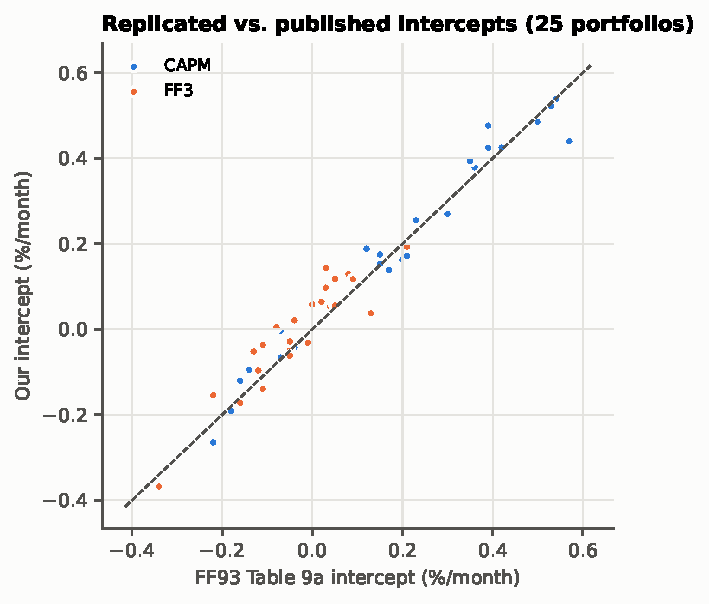
\includegraphics[width=\linewidth]{F05_intercepts_vs_ff93.pdf}\caption{Our intercepts vs.\ FF93 Table 9a.}\label{fig:F05_intercepts_vs_ff93}\end{subfigure}
\begin{subfigure}{0.48\linewidth}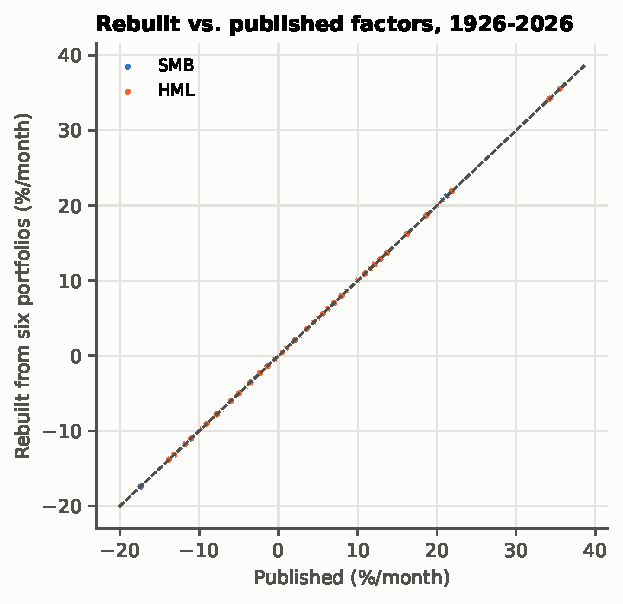
\includegraphics[width=\linewidth]{F02_factor_reconstruction.pdf}\caption{Rebuilt vs.\ published SMB/HML.}\label{fig:F02_factor_reconstruction}\end{subfigure}
\caption{Replication accuracy.}
\end{figure}

\begin{table}[H]\centering\small
\caption{Cell-by-cell agreement with FF93 (25 portfolios, 1963--1991).}\label{tab:agree}
\input{\tabdir/T05_replication_agreement.tex}
\end{table}

\paragraph{GRS tests.} Table~\ref{tab:grs} reports GRS statistics. In-sample, CAPM gives $F=\GrsCapmIS$ ($p=\GrsCapmISp$) and FF3 $F=\GrsFfIS$ ($p=\GrsFfISp$), against FF93's 1.91 and 1.56. FF93 used 32 assets including seven bond portfolios we cannot obtain, so the comparison is approximate. The ranking is the same: TERM+DEF ($\GrsTdIS$) worst, then CAPM, then SMB+HML, with FF3 best. Adding TERM and DEF to FF3 does not lower $F$ ($\GrsFfTdIS$), consistent with FF93's finding that bond factors add little for stocks. Figure~\ref{fig:F06_actual_vs_predicted_is} shows the same result as average returns plotted against model-implied returns. H1 is supported.

\begin{table}[H]\centering\small
\caption{GRS tests of zero intercepts on the 25 size/BE-ME portfolios. FF93 column: their Table 9c (32 assets).}\label{tab:grs}
\resizebox{\linewidth}{!}{\input{\tabdir/T06_grs_tests.tex}}
\end{table}

\begin{table}[H]\centering\small
\caption{Bond-factor proxies, 1963--1991 (FF93: TERM mean 0.06, SD 3.02; DEF mean 0.02, SD 1.60).}\label{tab:bond}
\input{\tabdir/T07_bond_factor_proxies.tex}
\end{table}

% =====================================================================
\section{Results: the strategy and its raw performance}

Figure~\ref{fig:F01_factor_cumulative} shows the factors' cumulative returns. Figure~\ref{fig:F08_strategy_cumulative} compares the strategies with the market. From \StartImom{} to \EndSample, industry momentum earns \ImomMean\% per year with volatility \ImomVol\% (Sharpe \ImomSharpe; market \MktSharpe), $t=\ImomT$, skewness \ImomSkew{} and a maximum drawdown of \ImomMaxDD\%. Its market beta is \ImomMktBetaCapm. Average one-way turnover is \Turnover\% of the long-plus-short book per month. At \CostBps{} bp the net return is \ImomNetMean\% (Sharpe \ImomNetSharpe). The long leg beats the market and the short leg lags it (Figure~\ref{fig:F09_strategy_legs}; Table~\ref{tab:perf}). The deepest drawdowns occur in 2001--2003 and in the 2009 momentum crash (a single-month loss of 34\% in April 2009) (Figure~\ref{fig:F10_drawdowns}). H3 is supported on raw returns.

\fig{F01_factor_cumulative}{Cumulative factor returns, July 1963--\EndSample{} (log scale). Shaded: NBER recessions.}
\fig{F08_strategy_cumulative}{Strategies vs.\ the market. ``Ex-ante hedged'' removes factor exposure estimated on trailing 60-month data only.}
\fig[0.8]{F09_strategy_legs}{Industry-momentum long and short legs (excess of T-bill).}
\fig[0.85]{F10_drawdowns}{Drawdowns from the running peak.}

\begin{table}[H]\centering\small
\caption{Performance summary by period (annualised). IS: 1963-07 to 1991-12; OOS: 1992-01 onward.}\label{tab:perf}
\resizebox{\linewidth}{!}{\input{\tabdir/T08_performance.tex}}
\end{table}

% =====================================================================
\section{Factor attribution}

\paragraph{The neutralisation ladder.} Table~\ref{tab:reg} is the paper's central result. The CAPM alpha is \ImomCapmAlpha\% per year ($t=\ImomCapmT$). FF3 alpha is \emph{larger}, \ImomFfAlpha\% ($t=\ImomFfT$), because the strategy loads negatively on HML (\ImomHmlBetaFf): past-winner industries tend to be growth industries, and HML had a positive premium. Under FF3 alone the strategy looks like outstanding alpha with $R^2$ of \ImomFfR. Adding UMD changes the picture. The UMD loading is \ImomUmdBeta{} ($t\approx30$), $R^2$ jumps to \ImomFfUmdR, and alpha falls to \ImomFfUmdAlpha\% ($t=\ImomFfUmdT$) under FF3+UMD and \ImomFfiveUmdAlpha\% ($t=\ImomFfiveUmdT$) under FF5+UMD (Figures~\ref{fig:F11_alpha_by_model}--\ref{fig:F12_imom_loadings}).

\begin{table}[H]\centering\small
\caption{Industry momentum (gross), July 1963--\EndSample. Coefficients with Newey--West $t$-statistics in parentheses; alpha in \% per year.}\label{tab:reg}
\resizebox{\linewidth}{!}{\input{\tabdir/P_regressions_imom.tex}}
\end{table}

\fig{F11_alpha_by_model}{Alpha shrinks as known factors are added. Industry momentum loses about three-quarters of its alpha once UMD enters. The small-value tilt loses most of its CAPM alpha once SMB and HML enter.}
\fig{F12_imom_loadings}{Industry-momentum loadings by model (95\% Newey--West confidence intervals).}

\paragraph{Risk decomposition and return attribution.} Decomposing variance as $\mathrm{Var}(r)=\beta'\Sigma_f\beta+\sigma^2_\varepsilon$, with Euler shares $\beta_k(\Sigma_f\beta)_k/\mathrm{Var}(r)$, UMD accounts for \UmdVarShare\% of industry-momentum variance and the residual for \ResidVarShare\% (Figure~\ref{fig:F17_risk_decomposition}). For the mean, UMD exposure contributes \UmdContribution{} percentage points per year of the \ImomMean\% average return (Figure~\ref{fig:F18_attribution_imom}). Figure~\ref{fig:F16_residual_returns} splits the cumulative return into a factor-explained part and an alpha-plus-residual part; the latter is small and noisy.

\fig[0.85]{F17_risk_decomposition}{Share of industry-momentum return variance by source.}
\begin{figure}[H]\centering
\begin{subfigure}{0.49\linewidth}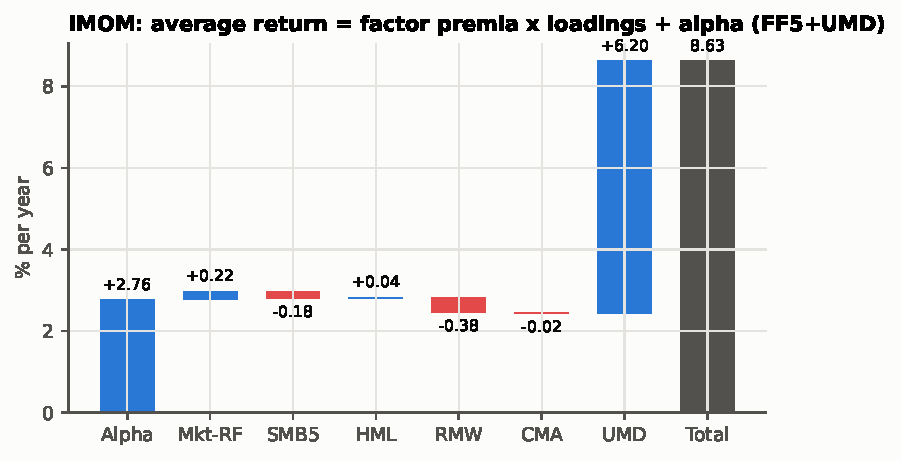
\includegraphics[width=\linewidth]{F18_attribution_imom.pdf}\caption{Industry momentum, FF5+UMD.}\label{fig:F18_attribution_imom}\end{subfigure}
\begin{subfigure}{0.49\linewidth}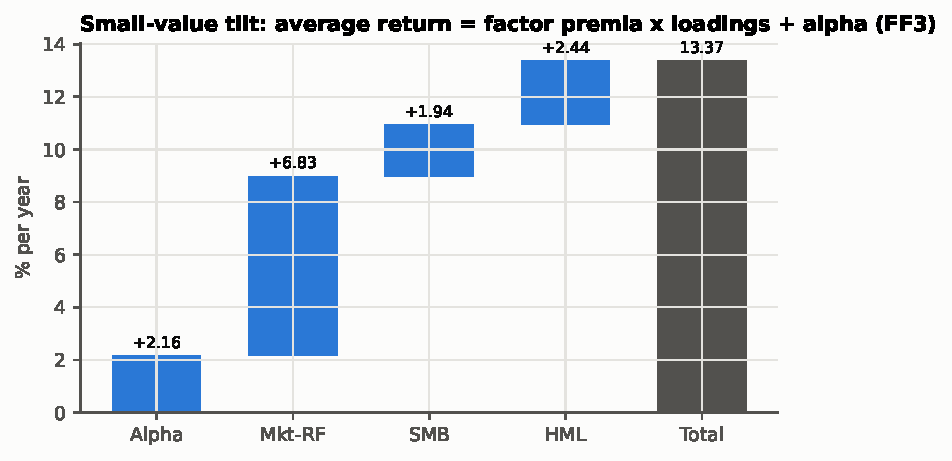
\includegraphics[width=\linewidth]{F18_attribution_smallvalue.pdf}\caption{Small-value tilt, FF3.}\label{fig:F18_attribution_smallvalue}\end{subfigure}
\caption{Average return = $\sum_k\beta_k\bar f_k + \alpha$ (\% per year).}
\end{figure}
\fig{F16_residual_returns}{Industry momentum split into its FF5+UMD factor-explained component and alpha + residual.}

\paragraph{Rolling exposures.} Sixty-month rolling regressions (Figures~\ref{fig:F13_rolling_betas}--\ref{fig:F14_rolling_alpha}) show that the UMD loading is persistently high, while market and value loadings swing. The rolling FF3+UMD alpha band includes zero for most of the sample. The rolling CAPM alpha is largest in the 1970s and remains positive afterwards, so the CAPM would have flagged ``alpha'' throughout.

\fig{F13_rolling_betas}{Rolling 60-month FF3+UMD betas of industry momentum.}
\fig{F14_rolling_alpha}{Rolling 60-month alpha (\% per year) with $\pm1.96$ standard-error bands.}

\paragraph{Ex-ante hedging.} The tradable factor-neutral version earns \HedMean\% per year with volatility \HedVol\% (Sharpe \HedSharpe). Its FF5+UMD alpha is \HedFfiveUmdAlpha\% ($t=\HedFfiveUmdT$; Table~\ref{tab:reghed}), and the hedge leaves near-zero realised loadings (Figure~\ref{fig:F19_hedge_effectiveness}). Neutralising the exposures removes the return they earned. What is left is the same small, marginal alpha.

\begin{table}[H]\centering\small
\caption{Ex-ante hedged industry momentum. Newey--West $t$-statistics in parentheses.}\label{tab:reghed}
\resizebox{\linewidth}{!}{\input{\tabdir/P_regressions_hedged.tex}}
\end{table}
\fig{F19_hedge_effectiveness}{Realised 36-month betas before and after the ex-ante hedge.}

\paragraph{Spanning in both directions.} A regression of industry momentum on UMD cannot tell which is more primitive. \citet{MG1999} argued that industry momentum drives stock momentum. Table~\ref{tab:span} runs the regression both ways. UMD's alpha against FF3+industry momentum is \UmdOnImomAlphaFull\% per year ($t=\UmdOnImomTFull$) over the full sample, about as fragile as industry momentum's alpha against UMD. The two strategies are largely the same risk, and neither robustly spans the other. Our evidence identifies the shared exposure, not its direction.

\begin{table}[H]\centering\small
\caption{Spanning tests in both directions (Newey--West $t$).}\label{tab:span}
\input{\tabdir/T20_spanning_both_directions.tex}
\end{table}

\paragraph{The control: a small-value tilt.} The smallest-size, highest-BE/ME portfolio earns \SvMean\% per year in excess of bills, with CAPM beta \SvMktBetaCapm{} and CAPM alpha \SvCapmAlpha\% ($t=\SvCapmT$). Its FF3 loadings are \SvSmbBeta{} on SMB and \SvHmlBeta{} on HML (Table~\ref{tab:regsv}; Figure~\ref{fig:F15_rolling_betas_smallvalue}). Over the full sample, FF3 cuts alpha to \SvFfAlpha\% ($t=\SvFfT$). The full-sample number hides a sharp split that Section~\ref{sec:oos} documents.

\begin{table}[H]\centering\small
\caption{Small-value tilt (S1B5 excess return), July 1963--\EndSample. Newey--West $t$ in parentheses.}\label{tab:regsv}
\resizebox{\linewidth}{!}{\input{\tabdir/P_regressions_smallvalue.tex}}
\end{table}
\fig{F15_rolling_betas_smallvalue}{Rolling 60-month FF3 betas of the small-value tilt.}

% =====================================================================
\section{Robustness}

\paragraph{Subperiods and the pre-1963 sample.} Table~\ref{tab:sub} splits the sample. The CAPM and FF3 alphas are large in every period. The UMD-controlled alpha is insignificant in every subperiod, including 1927--1963, where industry momentum earns \PreMean\% per year but its FF3+UMD alpha is \PreAlphaFfUmd\% ($t=\PreTFfUmd$). Since 2000 the FF5+UMD alpha is \PostTwoKAlphaFfUmd\% ($t=\PostTwoKTFfUmd$). Excluding Januaries changes nothing.

\begin{table}[H]\centering\small
\caption{Subperiods (alpha in \% per year; Newey--West $t$).}\label{tab:sub}
\resizebox{\linewidth}{!}{\input{\tabdir/T13_subperiods.tex}}
\end{table}

\paragraph{Parameter grid.} Across \GridN{} variants (lookback 3/6/9/12 months, skip 0/1, 5 or 10 industries per leg; Figure~\ref{fig:F21_parameter_grid}, Table~\ref{tab:grid}), every Sharpe ratio is positive both IS and OOS. The IS and OOS rankings are correlated (Spearman $\rho=\GridRho$). The IS-best specification, \GridBest, earns an OOS Sharpe of \GridBestSharpeOOS{} (grid median \GridMedianSharpeOOS) and an OOS FF5+UMD alpha of \GridBestAlphaOOS\% ($t=\GridBestTOOS$). Our a-priori specification ranks \BaseRankIS{} of \GridN{} in-sample. The deflated Sharpe ratio of the IS-best variant is \DsrBest, against a skill-less benchmark Sharpe of \SrZero{} (annualised) for the best of \GridN{} trials. The \emph{raw premium} is therefore not a data-mining artefact. The \emph{alpha} is the problem.

\fig{F21_parameter_grid}{Annualised Sharpe ratio across the parameter grid, in-sample vs.\ out-of-sample.}
\begin{table}[H]\centering\small
\caption{Parameter grid: Sharpe ratios and FF5+UMD alphas (\% per year), IS and OOS.}\label{tab:grid}
\input{\tabdir/T14_parameter_grid.tex}
\end{table}

\paragraph{Trading costs.} Each basis point of one-way cost lowers the annual return by about 0.1 percentage points (Table~\ref{tab:cost}; Figure~\ref{fig:F22_transaction_costs}). The raw premium breaks even at about \BreakEvenMean{} bp. The FF5+UMD alpha breaks even at \BreakEvenAlpha{} bp, and loses 5\% significance at about \CostTwoSig{} bp. Under the base \CostBps{} bp, the FF5+UMD alpha is \NetFfiveUmdAlpha\% ($t=\NetFfiveUmdT$). Industry-level costs for large, liquid stocks plausibly lie in the 10--30 bp range over most of the sample, and higher before the 1990s. Any genuine residual alpha is therefore within trading costs.

\begin{table}[H]\centering\small
\caption{Industry momentum after one-way trading costs (alpha in \% per year).}\label{tab:cost}
\input{\tabdir/T15_transaction_costs.tex}
\end{table}
\fig[0.75]{F22_transaction_costs}{Net Sharpe and alpha $t$-statistics as costs rise. Dashed lines: $t=1.96$ and the \citet{HLZ2016} $t=3$ hurdle.}

\paragraph{Hedge window.} The ex-ante hedge with 36-, 60- or 120-month estimation windows gives FF5+UMD alphas between 1.7\% and 2.7\% per year, none with $t>2.1$ (Table~\ref{tab:hedgew}).

\begin{table}[H]\centering\small
\caption{Ex-ante hedge: sensitivity to the beta-estimation window.}\label{tab:hedgew}
\resizebox{0.9\linewidth}{!}{\input{\tabdir/T16_hedge_windows.tex}}
\end{table}

\paragraph{Regimes.} Ex-ante market states matter for the level of returns, as H6 predicts (Table~\ref{tab:reg6}; Figure~\ref{fig:F24_regime_exposures}). After 24-month market declines (\BearMonths{} months), industry momentum earns \BearMean\% per year, against \BullMean\% otherwise. In ex-ante high-volatility states it earns \HiVolMean\%, against \LoVolMean\%. The UMD loading is stable across regimes (\BearUmdBeta{} in bear states vs.\ \BullUmdBeta{}), so the regime dependence is shared with UMD itself, consistent with \citet{CGH2004} and \citet{DM2016}. The point estimate of FF3+UMD alpha is higher in bear states (\BearAlpha\% vs.\ \BullAlpha\%) but imprecise. We treat it as a hypothesis for future work, not a finding. NBER recession labels are known only ex-post and are used descriptively.

\begin{table}[H]\centering\small
\caption{Regime-conditional performance and FF3+UMD exposures. Bear and high-volatility labels use data through $t-1$ only.}\label{tab:reg6}
\resizebox{\linewidth}{!}{\input{\tabdir/T18_regimes.tex}}
\end{table}
\fig{F24_regime_exposures}{Industry-momentum factor exposures by regime (95\% Newey--West confidence intervals).}

\paragraph{Multiple testing.} We ran \NTests{} alpha tests on industry-momentum variants (Table in the repository, \texttt{T17}; Figure~\ref{fig:F23_multiple_testing}). Among the \NUmdTests{} tests whose benchmark includes UMD, \NUmdTwo{} exceed $t=1.96$, \NUmdThree{} exceed $t=3$, and \NUmdHolm{} survive Holm's correction. Among the \NCapmFfTests{} tests with momentum-blind benchmarks, \NCapmFfHolm{} survive Holm. The contrast is the paper's answer in one figure.

\fig{F23_multiple_testing}{Every alpha test we ran on industry momentum, sorted by $t$-statistic. Orange: benchmark includes UMD.}

% =====================================================================
\section{Out-of-sample analysis}\label{sec:oos}

\paragraph{The three-factor model after 1991.} The GRS test that FF3 marginally passes in-sample ($p=\GrsFfISp$) fails decisively after 1991 ($F=\GrsFfOOS$, $p<0.001$), and over the full sample ($F=\GrsFfFull$). FF5 also fails ($F=\GrsFfiveFull$; Table~\ref{tab:grs}). Figure~\ref{fig:F06_actual_vs_predicted_oos} shows why: model-implied returns cluster while realised returns disperse, with small-growth stocks far below the line.

\begin{figure}[H]\centering
\begin{subfigure}{0.49\linewidth}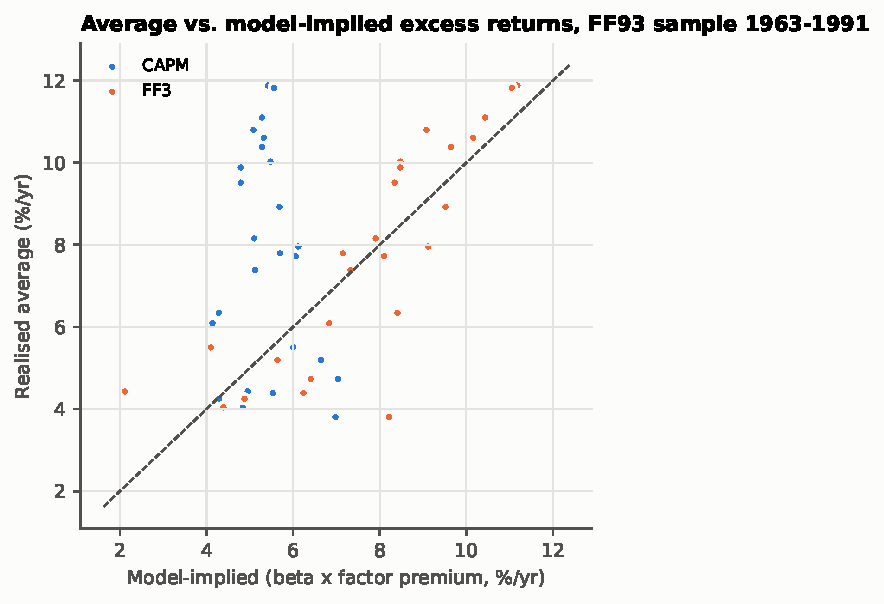
\includegraphics[width=\linewidth]{F06_actual_vs_predicted_is.pdf}\caption{1963--1991.}\label{fig:F06_actual_vs_predicted_is}\end{subfigure}
\begin{subfigure}{0.49\linewidth}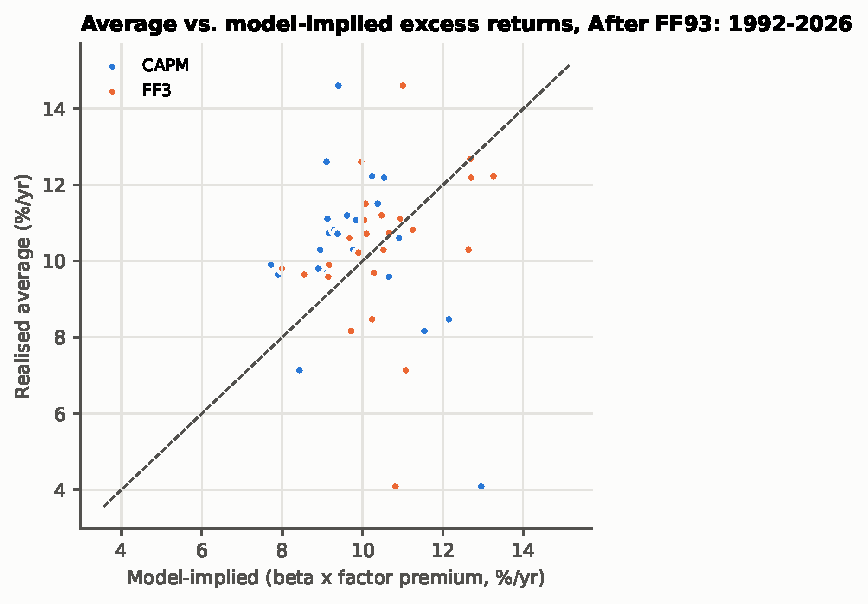
\includegraphics[width=\linewidth]{F06_actual_vs_predicted_oos.pdf}\caption{1992--2026.}\label{fig:F06_actual_vs_predicted_oos}\end{subfigure}
\caption{Average excess returns of the 25 portfolios vs.\ CAPM- and FF3-implied returns ($\hat\beta'\bar f$).}
\end{figure}

\paragraph{Strategies.} Table~\ref{tab:isoos} and Figure~\ref{fig:F20_is_vs_oos_imom} compare IS and OOS alphas. Industry momentum's raw Sharpe ratio falls from \ImomSharpeIS{} to \ImomSharpeOOS{} and its CAPM alpha from \ImomCapmAlphaIS\% to \ImomCapmAlphaOOS\%. That is the post-publication decay \citet{MP2016} document, and H5 is supported. The FF5+UMD alpha is insignificant in both halves (\ImomFfiveUmdAlphaIS\%, $t=\ImomFfiveUmdTIS$; \ImomFfiveUmdAlphaOOS\%, $t=\ImomFfiveUmdTOOS$), so the conclusion of H4 does not depend on the sample. The small-value tilt reverses the pattern (Figure~\ref{fig:F20_is_vs_oos_smallvalue}). In the FF93 sample, FF3 explains it almost completely (alpha \SvFfAlphaIS\%, $t=\SvFfTIS$; FF5+UMD \SvFfiveUmdAlphaIS\%). After 1991, an FF3 alpha of \SvFfAlphaOOS\% ($t=\SvFfTOOS$) appears. H2 holds in-sample only.

\begin{table}[H]\centering\small
\caption{Alpha (\% per year) in-sample (1963--1991) and out-of-sample (1992--2026); Newey--West $t$ in parentheses.}\label{tab:isoos}
\resizebox{0.8\linewidth}{!}{\input{\tabdir/P_is_vs_oos.tex}}
\end{table}
\begin{figure}[H]\centering
\begin{subfigure}{0.49\linewidth}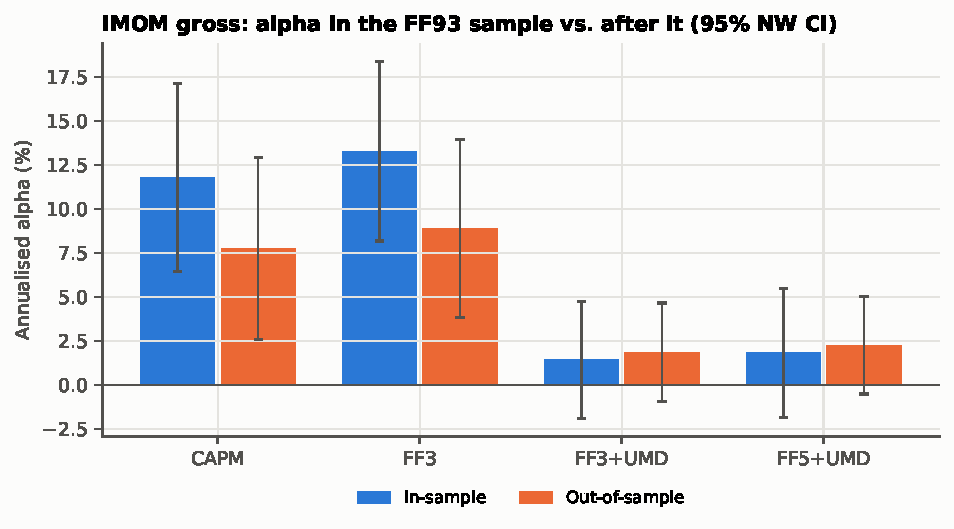
\includegraphics[width=\linewidth]{F20_is_vs_oos_imom.pdf}\caption{Industry momentum.}\label{fig:F20_is_vs_oos_imom}\end{subfigure}
\begin{subfigure}{0.49\linewidth}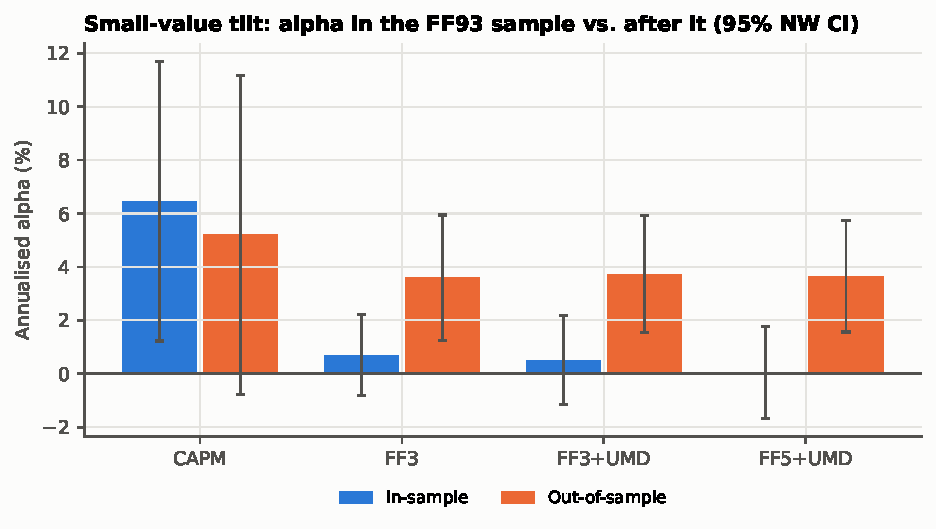
\includegraphics[width=\linewidth]{F20_is_vs_oos_smallvalue.pdf}\caption{Small-value tilt.}\label{fig:F20_is_vs_oos_smallvalue}\end{subfigure}
\caption{In-sample vs.\ out-of-sample alpha by model (95\% Newey--West confidence intervals).}
\end{figure}

\paragraph{International evidence.} With regional factors from \IntlStart{} (Table~\ref{tab:intl}; Figure~\ref{fig:F25_international}), the small-value tilt has a significant regional FF3 alpha in all \IntlNFfSig{} regions: Developed \DevFfAlpha\% ($t=\DevFfT$), North America \NaFfAlpha\% (\NaFfT), Europe \EurFfAlpha\% (\EurFfT), Japan \JpnFfAlpha\% (\JpnFfT), Asia Pacific ex Japan \ApxFfAlpha\% (\ApxFfT). FF3 $t$-statistics often \emph{exceed} the CAPM ones, because the factors remove so much noise that a smaller alpha becomes more precise. This is consistent with \citet{FF2012}, who find international value premiums that decrease with size and describe local factor models as only ``passable'' for size/BE-ME portfolios.

\begin{table}[H]\centering\small
\caption{Small-value tilt by region, July 1990--\EndSample{} (USD returns, regional factors).}\label{tab:intl}
\resizebox{\linewidth}{!}{\input{\tabdir/T19_international_smallvalue.tex}}
\end{table}
\fig{F25_international}{CAPM vs.\ regional FF3 alpha of the small-value tilt (95\% Newey--West confidence intervals).}

% =====================================================================
\section{Economic interpretation}

\paragraph{Industry momentum is a momentum-factor bet.} The strategy's apparent alpha has a simple explanation. It holds industries whose recent winners are the same stocks UMD buys, so it loads about 0.87 on UMD. UMD earned a large premium over the sample, so under any benchmark without UMD that premium looks like alpha. An investor could replicate two-thirds of the strategy's variance and most of its mean with a passive UMD position. Paying active fees for the strategy would be paying for a factor. Whether UMD itself is a risk premium or a persistent behavioural mispricing is a separate question. Our regressions cannot answer it, because a time-series alpha of zero is consistent with both interpretations \citep{DT1997}.

\paragraph{Neutrality is not free.} Hedging the factor exposures ex ante does exactly what it promises. The realised loadings go to roughly zero, and so does most of the return. Factor neutrality is a tool for isolating alpha, not for creating it.

\paragraph{A factor model is a sample-dependent benchmark.} The small-value control shows the other side. FF3 explains the small-value corner almost perfectly in the sample it was designed on, then leaves a 2--7\% annual alpha after 1991 and in every international region. ``Explained by factors'' is therefore a statement about a model in a sample. A strategy judged neutral today can show alpha against the same model tomorrow, and vice versa. Part of the post-1991 small-value alpha is probably not harvestable. The smallest NYSE size quintile contains thinly traded microcaps whose costs we do not model \citep{NMV2016}.

\paragraph{Correlation, not causation.} Every regression here measures co-movement and average returns. A UMD loading of 0.87 says industry momentum moves with stock momentum. It does not say UMD \emph{causes} its returns, and the two-way spanning tests confirm that the data cannot order them.

% =====================================================================
\section{Limitations}
\begin{itemize}
  \item \textbf{Portfolio-level data.} We trade industry portfolios, not stocks. Turnover inside industries, short-sale constraints and borrowing costs are ignored, so implementable returns are lower than reported.
  \item \textbf{Bond factors are proxies.} TERM and DEF come from monthly-average FRED yields with an assumed 20-year maturity. They match FF93's qualitative role but not its exact moments, and the seven bond test portfolios of FF93 are not available. Our GRS statistics therefore use 25 assets instead of 32.
  \item \textbf{Data revisions.} The French library revises history. Our numbers are tied to the \Vintage{} vintage and will drift slightly with later downloads; hashes are recorded.
  \item \textbf{Inference assumptions.} GRS assumes i.i.d.\ normal errors, which are rejected for monthly returns (fat tails, heteroskedasticity). Newey--West corrections are asymptotic. Constant betas within each regression window are an approximation.
  \item \textbf{Test assets.} The 25 size/BE-ME portfolios have a strong factor structure that flatters FF3 \citep{LNS2010}.
  \item \textbf{Researcher degrees of freedom.} We logged every alpha test, but choices of factor sets, windows and regime definitions are still ours. The OOS period is the only defence the data provide, and it is a single path.
  \item \textbf{A backtest is a hypothesis.} Nothing here establishes that any strategy will be profitable in the future.
\end{itemize}

% =====================================================================
\section{Conclusion}

We replicated \citet{FF1993} from public data with close agreement, then asked whether a simple industry-momentum strategy generates alpha or collects known factor premia. Against the CAPM and the three-factor model it looks like exceptional skill, with a 9--11\% annual alpha and $t$-statistics above 4.9. Against a benchmark that includes the momentum factor, alpha shrinks by about three-quarters. The remainder fails the $t>3$ hurdle and Holm's multiple-testing correction, is insignificant in each half of the sample and before 1963, and disappears after 25 bp trading costs. The strategy is, to a first approximation, a levered bet on momentum. The small-value control adds a caution. A factor model can explain an alpha in its own sample and fail outside it, so ``alpha versus factor exposure'' is a judgement that must be re-made out of sample.

\section{Future research}
\begin{itemize}
  \item Rebuild the analysis at the stock level (CRSP/Compustat) to measure true turnover, include short-sale costs and test whether \emph{within-industry} momentum carries alpha that industry momentum does not.
  \item Replace TERM and DEF proxies with total-return bond indices and add the seven FF93 bond portfolios to complete the 32-asset GRS test.
  \item Test conditional factor models in which betas depend on ex-ante market states, and momentum-crash hedges \citep{DM2016} as candidate sources of genuine alpha.
  \item Extend the factor-neutrality audit to international industry momentum and to other asset classes \citep{AMP2013}.
  \item Use bootstrap GRS and block-bootstrap alpha confidence intervals to relax normality.
\end{itemize}

\bibliographystyle{plainnat}
\bibliography{references}

\end{document}
